% Template for PLoS
% Version 1.0 January 2009
%
% To compile to pdf, run:
% latex plos.template
% bibtex plos.template
% latex plos.template
% latex plos.template
% dvipdf plos.template

\documentclass[10pt]{article}

% amsmath package, useful for mathematical formulas
\usepackage{amsmath}
% amssymb package, useful for mathematical symbols
\usepackage{amssymb}

% graphicx package, useful for including eps and pdf graphics
% include graphics with the command \includegraphics
\usepackage{graphicx}

% cite package, to clean up citations in the main text. Do not remove.
%\usepackage{cite} % removed to use natbib instead

\usepackage{color}

\usepackage{hyperref} % for urls

\usepackage{natbib}

\usepackage{kbordermatrix} % for labeling matrix rows and columns

% Use doublespacing - comment out for single spacing
%\usepackage{setspace} 
%\doublespacing

% Text layout
\topmargin 0.0cm
\oddsidemargin 0.5cm
\evensidemargin 0.5cm
\textwidth 16cm 
\textheight 21cm

% Bold the 'Figure #' in the caption and separate it with a period
% Captions will be left justified
\usepackage[labelfont=bf,labelsep=period,justification=raggedright]{caption}


% Remove brackets from numbering in List of References
\makeatletter
\renewcommand{\@biblabel}[1]{\quad#1.}
\makeatother


% Leave date blank
\date{}

\pagestyle{myheadings}
%% ** EDIT HERE **


%% ** EDIT HERE **
%% PLEASE INCLUDE ALL MACROS BELOW

%% END MACROS SECTION

\begin{document}

% Title must be 150 characters or less
\begin{flushleft}
{\Large
\textbf{Approximating multi-type birth-death likelihoods using local decoupling}
% OR
%\textbf{Phylodynamics with adaptive molecular evolution using fitness-dependent birth-death models}
}
\newline
% Insert Author names, affiliations and corresponding author email.
\\
David A. Rasmussen\textsuperscript{1,2*},
Shi Cen\textsuperscript{1,2}
\\
\bigskip
\textbf{1} Department of Entomology and Plant Pathology, North Carolina State University, Raleigh, North Carolina, USA\\
\textbf{2} Bioinformatics Research Center, North Carolina State University, Raleigh, North Carolina, USA\\
\bigskip

* E-mail: drasmus@ncsu.edu
\end{flushleft}

%%%%%%%%%%%
\section*{Introduction}

Blah blah blah...

\section*{Models and Methods}

\subsection*{The exact MTBD model}

%%%
 
% TEXT TAKEN FROM RASMUSSEN & STADLER (2019)
 
%%%

The multi-type birth-death (MTBD) model of \citet{stadler2013uncovering} can be used to exactly compute the joint likelihood $L(S,\mathcal{T} | \mu, \theta)$ of the sequence or character state data $\mathcal{S}$ and phylogenetic tree $\mathcal{T}$ in a way that couples the mutation process with changes in fitness along a lineage. Let $D_{n}(t)$ represent the probability density (i.e. the likelihood) that the subtree descending from lineage $n$ evolved between time $t$ and the present exactly as observed. Further, let $D_{n,i}(t)$ represent this probability density conditional on lineage $n$ being in state $i$ out of $M$ possible states at time $t$. Here the state of a lineage refers to a particular allele or character state (e.g. nucleotide or amino acid) at a single site. We reserve the term genotype to refer to a particular configuration of states across multiple sites in a sequence.

The density $D_{n,i}(t)$ can be computed going backwards in time from the present ($t=0$) to time $t$ along a lineage by numerically solving a system of ordinary differential equations:
\begin{eqnarray} \label{probD_ODE}
	\frac{d}{dt} D_{n,i}(t) = 
	-(\lambda_{i} + \sum_{j=1}^{M} \gamma_{i,j} + d_{i}) D_{n,i}(t) & & \text{(a) no event} \nonumber \\
	+ 2 \lambda_{i} E_{i}(t) D_{n,i}(t) & & \text{(b) birth of lineage with no sampled descendants} \\
	+ \sum_{j=1}^{M} \gamma_{i,j} D_{n,j}(t) & & \text{(c) mutation from $i$ to $j$}. \nonumber
\end{eqnarray}  
Here, $\lambda_{i}$ is the birth rate and $d_{i}$ is the death rate of lineages in state $i$, and thus reflect a lineage's fitness. Mutations between states $i$ and $j$ occur at a rate $\gamma_{i,j}$, independently of birth events. Each term in \eqref{probD_ODE} describes how $D_{n,i}$ changes through time by accounting for all of the different events that could have occurred along the lineage. The first term (a) considers the change in probability density given that no birth, death or mutation event occurred. The second term (b) considers the probability of a birth event that went unobserved because one of the child lineages produced no sampled descendants (this event has probability $E_{i}(t)$, see below). The third term (c) reflects the probability that the lineage mutated from state $i$ to $j$.

$E_{i}(t)$ represents the probability that a lineage in state $i$ is not sampled and has no sampled descendants. This probability can be computed at any time $t$ by solving a second set of ODEs:
\begin{eqnarray} \label{probE_ODE}
	\frac{d}{dt} E_{i}(t) = 
	(1 - s_{i}) d_{i} & & \text{(a) death without sampling} \nonumber \\
	- (\lambda_{i} + \sum_{j=1}^{M} \gamma_{i,j} + d_{i}) E_{i}(t) & & \text{(b) no event} \\
	+ \lambda_{i} E_{i}(t)^{2} & & \text{(c) birth, neither child has sampled descendants} \nonumber \\
	+ \sum_{j=1}^{M} \gamma_{i,j} E_{j}(t). & & \text{(d) mutation from $i$ to $j$} \nonumber
\end{eqnarray}
The first term (a) reflects the probability that a lineage dies and is not sampled, where $s_{i}$ is the probability that a lineage in state $i$ is sampled upon dying. Terms b-d have similar interpretations as in \eqref{probD_ODE}. 

At a tip lineage $n$, we initialize $D_{n,i}(t) = d_{i} s_{i}$ if the lineage was sampled upon death at time $t$. Alternatively, if $n$ was sampled at the present time $t=0$ before dying, then $D_{n,i}(t) = \rho_{i}$, where $\rho_{i}$ is the probability that an individual in state $i$ was sampled at present. At a branching event, the probability density $D_{a,i}$ of the parent lineage $a$ in state $i$ giving rise to two descendent lineages $n$ and $m$ is updated as:
\begin{equation} \label{pruning}
	D_{a,i} = 2 \lambda_{i} D_{m,i}(t) D_{n,i}(t).
\end{equation}  
The factor of two enters because either lineage $m$ or $n$ could have given birth and we must consider both possible events.

At the root, we can compute the probability density of the entire tree by summing over all possible root states:
\begin{equation} \label{rootDensity}
	D_{n} = \sum_{i=1}^{M} q_{i} \frac{D_{n,i}(t_{root})}{1 - E_{i}(t_{root})}, 
\end{equation}
where $q_{i}$ is the prior probability that the root is in state $i$ at time $t_{root}$. Including the term $1 - E_{i}(t_{root})$ in the denominator conditions the birth-death process on giving rise to at least one sampled individual.  $D_{n}$ represents the probability that the entire tree and the tip states $\mathcal{S}$ evolved as exactly as observed. It is therefore equivalent to the joint likelihood $L(\mathcal{S}, \mathcal{T} | \mu, \theta)$ we seek where $\mu = \{\gamma\}$ and $\theta = \{\lambda, d, s\}$.

%%%%%%%%%%%%%%%%%%%%%%
\subsection*{Numerical issues with the exact MTBD model}

Computing the likelihood of tree under the MTBD model as described above requires numerically integrating a system of differential equations along each branch or lineage in the tree. This creates a problem if we wish to auto-differentiate the likelihood function to compute derivatives of the likelihood function with respect to the model parameters in gradient-based inference methods like HMC. In that case we would need to repeatedly numerically integrate the ODEs while also numerically differentiating the likelihood function, which would be computationally inefficient. We therefore propose an approximation to the exact likelihood function below which more easily lends itself to auto-differentiation. 

%%%%%%%%%%%%%%%%%%%%%%
\subsection*{Approximating the MTBD likelihood through local decoupling}

We can approximate the probability densities for the exact MTBD model given in \eqref{probD_ODE} by locally ``decoupling'' the birth-death process giving rise to the tree from the Markov jump process that causes lineages to transition between states. Our approach is essentially a discrete-time approximation to the continuous-time MTBD model where over each time step we temporarily decouple the birth-death process from the state jump/transition process.

Again letting $D_{n,i}(t)$ denote the probability density of the subtree descending from lineage $n$ evolving as observed conditional on being in state $i$ at time $t$, we update $D_{n,i}(t)$ over a small time-step $\Delta t$ as:
\begin{equation} \label{approx_D_updatte}
	D_{n,i}(t + \Delta) = \bigg( \sum_{j=1}^{M} p_{i,j}(\Delta t) D_{n,i}(t) \bigg)  \hat{D}_{n,i}(\Delta t).
\end{equation}
Here, $p_{i,j}(\Delta t)$ is the probability that the lineage transitioned from state $i$ to state $j$ over the time step $\Delta t$; and $\hat{D}_{n,i}(\Delta t)$ is the approximate probability that the lineage evolved as observed under the birth-death model conditional on being in state $i$. We discuss how both of these probabilities are computed below. The updates follow a pattern similar to how state probabilities are updated under standard hidden Markov models (HMMs). We sum over all the ways a lineage in could transition to state $i$ from any other state $j$ according to the transition probabilities $p_{i,j}(\Delta t)$. We then complete the update by computing the ``emission'' probability  $\hat{D}_{n,i}(\Delta t)$ of observing the data, or in our case the tree, over the time step.

The transition probabilities $p_{i,j}(\Delta t)$ are computed as under a standard Markov jump process:
$$
	p_{i,j}(\Delta t) = e^{Q \Delta t},
$$
where $Q$ is the transition generator matrix corresponding to the transition rate matrix $\gamma$:
$$
Q =
\begin{bmatrix} 
	-\sum_{i \neq 1}^{M} \gamma_{1,i} & \gamma_{1,2} & \cdots & \gamma_{1,M} \\ 
	\gamma_{2,1} & -\sum_{i \neq 2}^{M} \gamma_{2,i} & \cdots & \gamma_{2,M} \\ 
	\vdots & \vdots & \ddots & \vdots \\ 
	\gamma_{M,1} & \gamma_{M,2} & \cdots & -\sum_{i \neq n}^{n} \gamma_{M,i} 
\end{bmatrix}
$$
Note that some MTBD models allow individuals to transition between states at birth/transmission events according to a birth rate matrix $\lambda$ with off-diagonal elements. This can be accommodated by summing the off-diagonal elements of  
$\gamma$ and $\lambda$ together to get the total rates at which lineage transition between states in $Q$.

Conditional on a lineage being in a given state $i$, the approximate probabilities $\hat{D}_{n,i}(\Delta t)$ of a lineage evolving as observed over the time step $\Delta t$ under a single-type birth-death model are described in \citet{barido2018detection}. These probabilities are approximate not only because they assume the lineage itself cannot transition between states over $\Delta t$, but also because they assume any unsampled lineages that lineage $n$ gave raise to also remain in state $i$. 

%\subsubsection*{Computing state probabilities from $D_{n,,i}$}

% This might be useful to save

%In our notation, $\omega_{n,k,i}$ represents the conditional probability $p(i | \mathcal{T}_{n}, \mathcal{S}_{n})$ that lineage $n$ is in particular state $i$, where $\mathcal{T}_{n}$ represents the subtree descending from $n$ with tip sequences $\mathcal{S}_{n}$. $D_{n,k,i}$ represents the inverse conditional probability density $p(\mathcal{T}_{n}, \mathcal{S}_{n} | i)$. We can therefore apply Bayes theorem to compute $\omega_{n,k,i}$ given $D_{n,k,i}$:
%\begin{equation} \label{normalizedStateProbs}
%	\omega_{n,k,i} = p(i | \mathcal{T}_{n}, \mathcal{S}_{n}) = \frac{p(\mathcal{T}_{n}, \mathcal{S}_{n} | i) q(i)}{\sum_{i}^{M} p(\mathcal{T}_{n}, \mathcal{S}_{n} | i) q(i)} = \frac{D_{n,k,i} q(i)}{\sum_{i}^{M} D_{n,k,i} q(i)}.
%\end{equation}
%The $q(i)$ terms represent the prior probability that the lineage is in state $i$. Here we make a simplification in assuming that the tree ancestral and sister to lineage $n$ has no information regarding $\omega_{n,k,i}$, and thus assume a uniform prior on $q(i)=1/M$. The $q(i)$ terms therefore cancel above.


%%%%%%%%%
\section*{Results}

\subsubsection*{Testing the approximation}

We first tested our local decoupling approximation against the exact MTBD model of \citet{stadler2013uncovering} by considering the probability densities $D_{n,i}(t)$ for a single lineage evolving backwards in time. For a simple model with four states, Figure~\ref{fig:approx_test}A-B show that there is quite good agreement between the probability densities computed under the approximate and exact model. We also considered the probability of the lineage being in each state backwards in time under both models, which are likewise highly condcordant.

% Figure 1
\begin{figure}[!h]
	\centering
	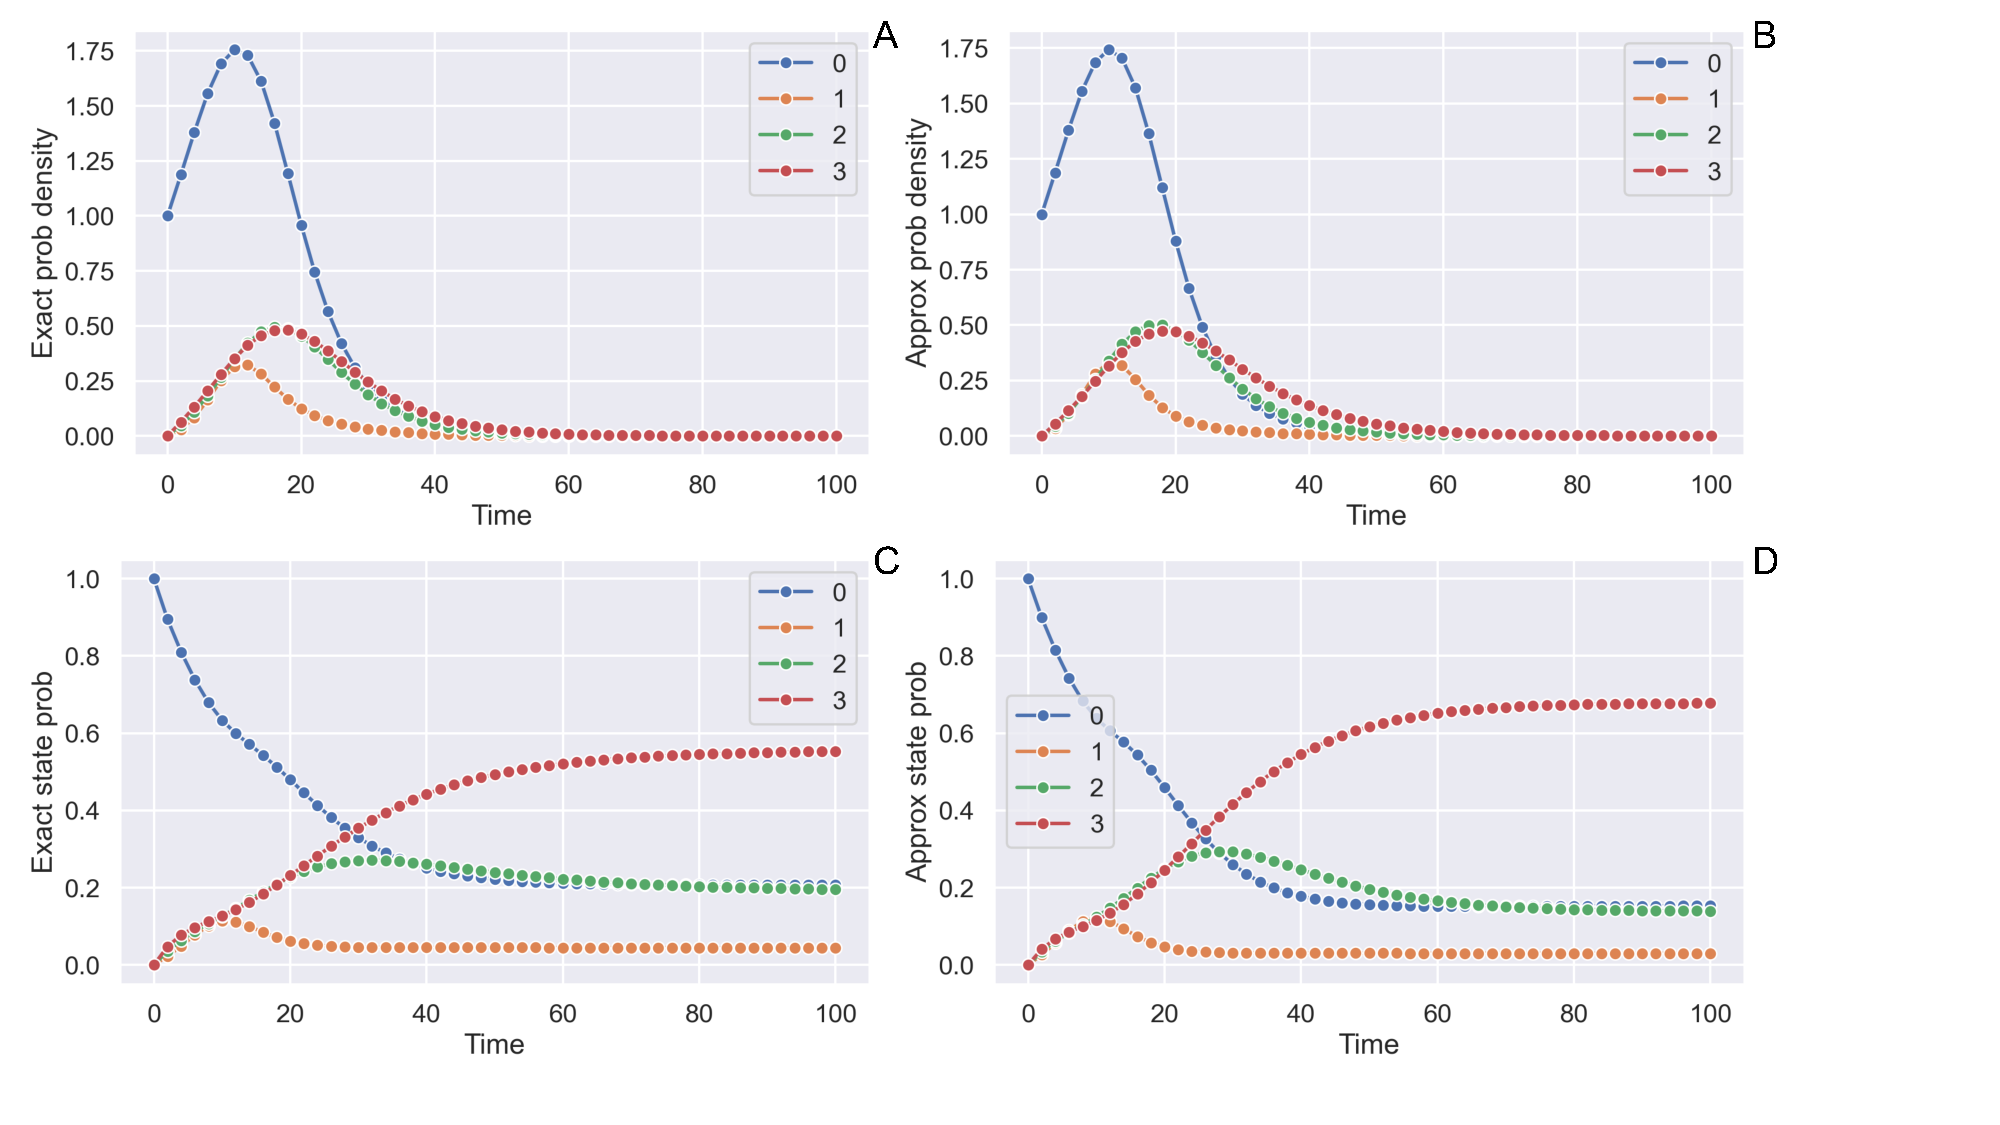
\includegraphics[width=1.0\linewidth]{./mtbd_approx_vs_exact}
	\caption{{\bf Testing the local decoupling approximation against exact MTBD model.} \textbf{(A-B)} Exact versus approximate probability densities $D_{n,i}(t)$ conditional on each of the four states. \textbf{(C-D)} Exact versus approximate lineage probabilities.}
	\label{fig:approx_test}
\end{figure}

\bibliographystyle{abbrvnat}
\bibliography{fitnessBirthDeathRefs} % The bibtex filename

%\newpage
%\section*{Figures}

\end{document}

